% ------------------------------------------------------------------------------
% TYPO3 CMS 6.2 LTS - What's New - Chapter "Install Tool" (Spanish Version)
%
% @author	Sergio Catalá <sergio.catala@e-net.info>
% @author	Michel Mix <mmix@autistici.org>
% @license	Creative Commons BY-NC-SA 3.0
% @link		http://typo3.org/download/release-notes/whats-new/
% @language	Spanish
% ------------------------------------------------------------------------------
% Chapter: Install Tool
% ------------------------------------------------------------------------------

\section{Herramienta de Instalación}
\begin{frame}[fragile]
	\frametitle{Herramienta de Instalación}

	\begin{center}\huge{Capítulo 1:}\end{center}
	\begin{center}\huge{\color{typo3darkgrey}\textbf{La Herramienta de Instalación}}\end{center}

\end{frame}

% ------------------------------------------------------------------------------
% Installation
% ------------------------------------------------------------------------------

\begin{frame}[fragile]
	\frametitle{Herramienta de Instalación}
	\framesubtitle{Instalación (1)}

	\begin{itemize}
		\item Sólo se requiere \underline{un} paquete para una instalación:\newline
				\texttt{typo3\_src-6.2.x.tar.gz} (tamaño del fichero: aprox. 20MB)
		\item Los paquetes "Dummy" y "Blank" quedaron obsoletos
		\item Instalación:
			\begin{itemize}
				\item El paquete fuente se extrae en el directorio web raíz
				\item Se crean los enlaces simbólicos requeridos
				\item Apunte el navegador web a su directorio raíz
				\item El Instalador de TYPO3 empieza el asistente de 1-2-3-4-pasos
			\end{itemize}

	\end{itemize}

\end{frame}

% ------------------------------------------------------------------------------
% Installation
% ------------------------------------------------------------------------------

\begin{frame}[fragile]
	% \TabPositions{2cm}

	\frametitle{Herramienta de Instalación}
	\framesubtitle{Instalación (2)}

	\begin{itemize}
		\item El instalador se asegura de que todos los ficheros y directorios necesarios estén en su sitio
		\item Se crearán automáticamente los ficheros necesarios para una configuración personalizada
		\item Los siguientes enlaces simbólicos \underline{deben} existir:

		\begin{itemize}
			\item \texttt{typo3\_src}	\tabto{2cm} (apunta al directorio raíz de TYPO3)
			\item \texttt{typo3}		\tabto{2cm} (apunta al directorio: \texttt{typo3\_src/typo3})
			\item \texttt{index.php}	\tabto{2cm} (apunta al fichero: \texttt{typo3\_src/index.php})
		\end{itemize}

		\item ¡No se requieren más ficheros/directorios para instalar TYPO3!
		\item Directorio \texttt{t3lib} eliminado
		\item Más detalles: Guía de Instalación y Actualización de TYPO3\newline
			\url{http://docs.typo3.org/typo3cms/InstallationGuide}

	\end{itemize}

\end{frame}

% ------------------------------------------------------------------------------
% Re-Development
% ------------------------------------------------------------------------------

\begin{frame}[fragile]
	\frametitle{Herramienta de Instalación}
	\framesubtitle{Redesarrollo (1)}

	\begin{columns}[T]

		\begin{column}{.5\textwidth}
			\begin{itemize}
				\item Redesarrollado desde cero usando Fluid
				\item El \underline{primer} paso chequea el entorno del sistema y reporta asuntos
				\item Los asuntos reportados pueden arreglarse\newline (y re-testearse) o ignorarse
			\end{itemize}
		\end{column}

		\begin{column}{.5\textwidth}
			\begin{figure}\vspace*{-0.4cm}
				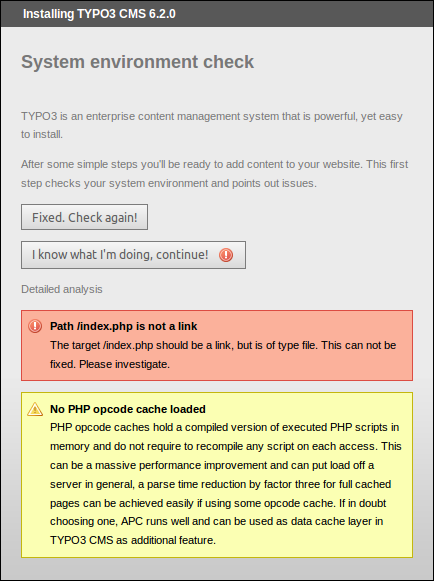
\includegraphics[width=0.8\linewidth]{Images/InstallTool/SystemEnvironmentCheck.png}
			\end{figure}
		\end{column}

	\end{columns}

\end{frame}

% ------------------------------------------------------------------------------
% Re-Development
% ------------------------------------------------------------------------------

\begin{frame}[fragile]
	\frametitle{Herramienta de Instalación}
	\framesubtitle{Redesarrollo (2)}

	\begin{columns}[T]

		\begin{column}{.5\textwidth}
			\begin{itemize}
				\item La configuración inválida del núcleo (p.ej. no enlaces simbólicos como se recomienda) se reporta como un asunto, también
			\end{itemize}
		\end{column}

		\begin{column}{.5\textwidth}
			\begin{figure}\vspace*{-0.4cm}
				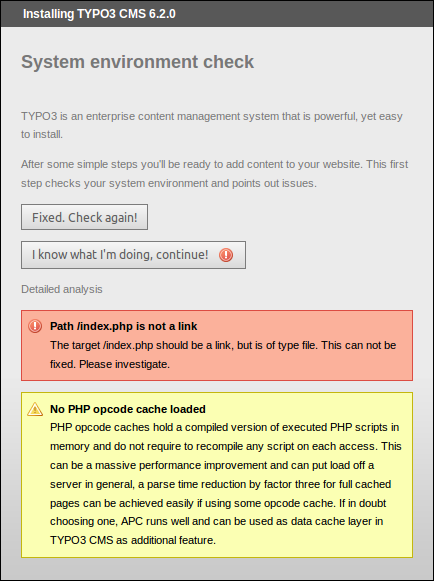
\includegraphics[width=0.8\linewidth]{Images/InstallTool/SystemEnvironmentCheck.png}
			\end{figure}
		\end{column}

	\end{columns}

\end{frame}

% ------------------------------------------------------------------------------
% Re-Development
% ------------------------------------------------------------------------------

\begin{frame}[fragile]
	\frametitle{Herramienta de Instalación}
	\framesubtitle{Redesarrollo (3)}

	\begin{columns}[T]

		\begin{column}{.5\textwidth}
			\begin{itemize}
				\item El \underline{segundo} paso permite a los usuarios introducir los detalles de acceso a la base de datos
				\item Se pueden seleccionar tipos de conexión
					\begin{itemize}
						\item Conexión basada en TCP/IP
						\item Conexión basada en Socket
					\end{itemize}
				\item Son también posibles alternativas a MySQL
			\end{itemize}
		\end{column}

		\begin{column}{.5\textwidth}
			\begin{figure}\vspace*{-0.4cm}
				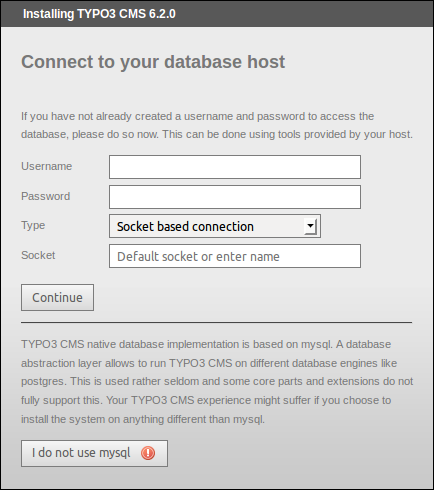
\includegraphics[width=0.8\linewidth]{Images/InstallTool/DatabaseConnectionDetails.png}
			\end{figure}
		\end{column}

	\end{columns}

\end{frame}

% ------------------------------------------------------------------------------
% Re-Development
% ------------------------------------------------------------------------------

\begin{frame}[fragile]
	\frametitle{Herramienta de Instalación}
	\framesubtitle{Redesarrollo (4)}

	\begin{columns}[T]

		\begin{column}{.5\textwidth}
			\begin{itemize}
				\item El \underline{tercer} paso permite a los usuarios seleccionar/crear la base de datos\newline
					(como en TYPO3 < 6.2)
				\item El \underline{cuarto} paso permite a los usuarios fijar una contraseña para el usuario "admin"\newline (que es también la contraseña inicial de la Herramienta de Instalación) y un nombre para el sitio
			\end{itemize}
		\end{column}

		\begin{column}{.5\textwidth}
			\begin{figure}\vspace*{-0.4cm}
				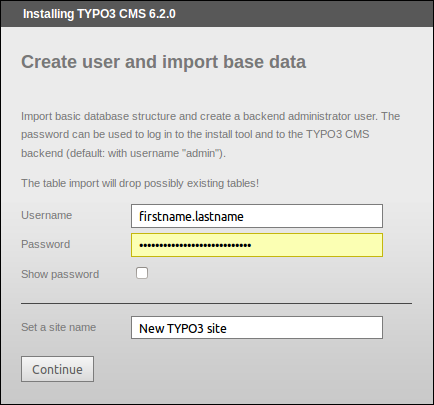
\includegraphics[width=0.8\linewidth]{Images/InstallTool/AdminPasswordAndSiteName.png}
			\end{figure}
		\end{column}

	\end{columns}

\end{frame}

% ------------------------------------------------------------------------------
% Delete All Cache
% ------------------------------------------------------------------------------

\begin{frame}[fragile]
	\frametitle{Herramienta de Instalación}
	\framesubtitle{Borrar Toda la Caché (1)}

	\begin{itemize}
		\item Nueva función bajo "Acciones importantes" permite a los usuarios borrar toda la caché
		\item Esto también funciona, si la caché contiene código PHP inválido\newline
			(lo que posiblemente bloquee TYPO3 CMS)
		\item Se puede evitar una instancia TYPO3 que no funciona accediendo a la Herramienta de Instalación directamente: \texttt{http://example.com/typo3/install}
	\end{itemize}

	\begin{columns}[T]
		\begin{column}{.3\textwidth}
			\begin{figure}\vspace*{-0.4cm}
				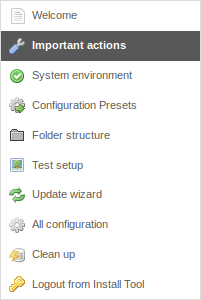
\includegraphics[width=0.7\linewidth,height=3cm]{Images/InstallTool/ImportantActions.png}
			\end{figure}
		\end{column}
		\begin{column}{.7\textwidth}
			\begin{figure}\vspace*{-0.4cm}
				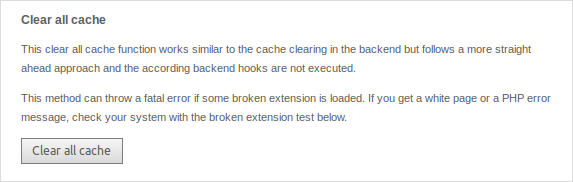
\includegraphics[width=0.9\linewidth]{Images/InstallTool/ClearAllCache.png}
			\end{figure}
		\end{column}
	\end{columns}

\end{frame}

% ------------------------------------------------------------------------------
% Delete All Cache
% ------------------------------------------------------------------------------

\begin{frame}[fragile]
	\frametitle{Herramienta de Instalación}
	\framesubtitle{Borrar Toda la Caché (2)}

	Secuencia de acciones al ejecutar "Borrar toda la caché":

	\begin{enumerate}
		\item Se borra el contenido del directorio \texttt{typo3temp/Cache}
		\item Se vacían las tablas \texttt{cf\_*} de la base de datos
		\item Se cargan los ficheros \texttt{ext\_localconf.php} y \texttt{ext\_tables.php}\newline
			de las extensiones
		\item Se ejecuta \texttt{flushCaches()}
	\end{enumerate}

\end{frame}

% ------------------------------------------------------------------------------
% Check For Broken Extensions
% ------------------------------------------------------------------------------

\begin{frame}[fragile]
	\frametitle{Herramienta de Instalación}
	\framesubtitle{Chequeo de Extensiones Rotas}

	\begin{itemize}
		\item Nueva función bajo "Acciones importantes" deja a los usuarios chequear, si se pueden cargar extensiones sin romper el sistema
		\item Muy útil para una actualización de TYPO3 4.5 a 6.2
	\end{itemize}

	\begin{columns}[T]
		\begin{column}{.3\textwidth}
			\begin{figure}\vspace*{-0.4cm}
				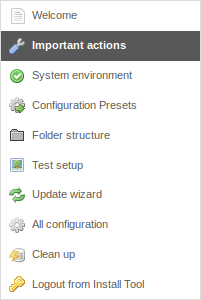
\includegraphics[width=0.7\linewidth]{Images/InstallTool/ImportantActions.png}
			\end{figure}
		\end{column}
		\begin{column}{.7\textwidth}
			\begin{figure}\vspace*{-0.4cm}
				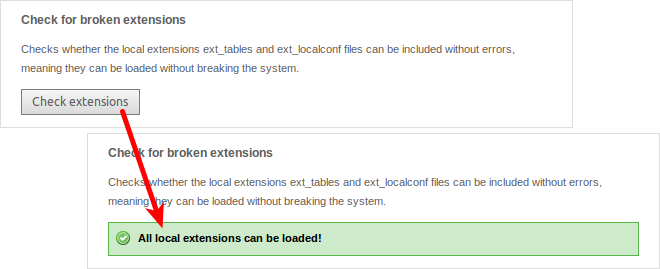
\includegraphics[width=1\linewidth]{Images/InstallTool/CheckForBrokenExtensions.png}
			\end{figure}
		\end{column}
	\end{columns}

\end{frame}

% ------------------------------------------------------------------------------
% Increased Security: Salted Passwords
% ------------------------------------------------------------------------------

\begin{frame}[fragile]
	\frametitle{Herramienta de Instalación}
	\framesubtitle{Contraseñas Salted}

	\begin{itemize}
		\item Al crear el nuevo usuario administrador del backend vía la Herramienta de Instalación, se usa una contraseña \textbf{salted}\newline
			\smaller(requiere que esté instalada, cargada y configurada EXT:saltedpasswords)\normalsize
		\item La contraseña de la Herramienta de Instalación es una contraseña \textbf{salted} también
			\smaller(los MD5 hashes existentes se convierten automáticamente en el primer inicio de sesión)\normalsize
	\end{itemize}

	\begin{columns}[T]
		\begin{column}{.3\textwidth}
			\begin{figure}\vspace*{-0.4cm}
				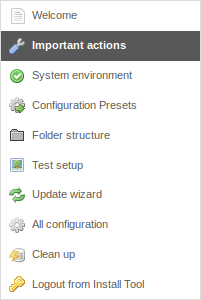
\includegraphics[width=0.7\linewidth]{Images/InstallTool/ImportantActions.png}
			\end{figure}
		\end{column}
		\begin{column}{.7\textwidth}
			\begin{figure}\vspace*{-0.4cm}
				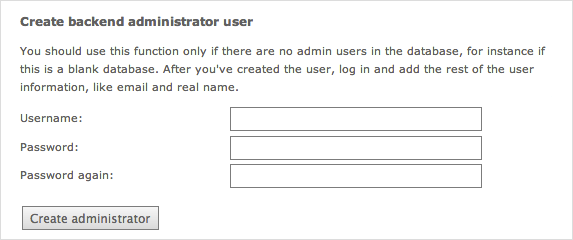
\includegraphics[width=0.9\linewidth]{Images/InstallTool/SaltedPasswords.png}
			\end{figure}
		\end{column}
	\end{columns}

\end{frame}

% ------------------------------------------------------------------------------
% Application Context
% ------------------------------------------------------------------------------

\begin{frame}[fragile]
	\frametitle{Herramienta de Instalación}
	\framesubtitle{Contexto de la Aplicación}

	\begin{itemize}
		\item TYPO3 >= 6.2 tiene en cuenta el \textbf{Contexto de la Aplicación}\newline
			\smaller(conocido en TYPO3 Flow)\normalsize
		\item La variable de entorno \texttt{TYPO3\_CONTEXT} fija el contexto\newline
			\smaller(por defecto: \texttt{Production}, subcontexto tal como \texttt{Production/Staging} posible)\normalsize

			\begin{lstlisting}
				# Fichero: .htaccess
				# Reglas para fijar el Contexto basada en el nombre del host:

				RewriteCond %{HTTP_HOST} ^dev\.example\.com$
				RewriteRule (.*) $1 [E=TYPO3_CONTEXT:Development]

				RewriteCond %{HTTP_HOST} ^www\.example\.com$
				RewriteRule (.*) $1 [E=TYPO3_CONTEXT:Production]

				# Fija una variable de entorno, disponible ahora en TYPO3 CMS:
				SetEnv TYPO3_CONTEXT Production
			\end{lstlisting}

	\end{itemize}

\end{frame}

% ------------------------------------------------------------------------------
% Application Context
% ------------------------------------------------------------------------------

\begin{frame}[fragile]
	\frametitle{Herramienta de Instalación}
	\framesubtitle{Presets de Ajustes en TYPO3\_CONF\_VAR (1)}

	\begin{columns}[T]
		\begin{column}{.5\textwidth}

			\begin{itemize}
				\item Ciertos ajustes \texttt{TYPO3\_CONF\_VAR} pueden configurarse en la Herramienta de Instalación
				\item Ajustes como la salida de depuración, el registro de discontinuación, devIPmask y otros registros del sistema y niveles de registro
			\end{itemize}

		\end{column}
		\begin{column}{.5\textwidth}

			\begin{figure}\vspace*{-0.4cm}
				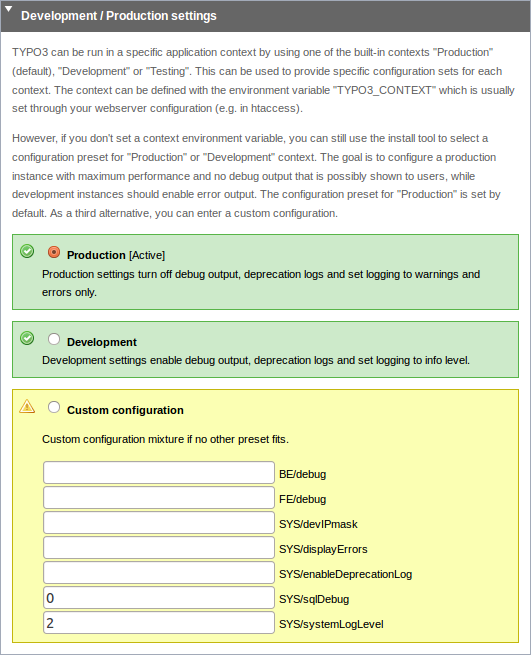
\includegraphics[width=0.8\linewidth]{Images/InstallTool/ApplicationContext.png}
			\end{figure}

		\end{column}
	\end{columns}

\end{frame}

% ------------------------------------------------------------------------------
% Application Context
% ------------------------------------------------------------------------------

\begin{frame}[fragile]
	\frametitle{Herramienta de Instalación}
	\framesubtitle{Presets de Ajustes en TYPO3\_CONF\_VAR (2)}

	\begin{columns}[T]
		\begin{column}{.5\textwidth}

			\begin{itemize}
				\item Contextos incorporados: "Production" y "Development"\newline
					(es posible una configuración personalizada)
			\end{itemize}

		\end{column}
		\begin{column}{.5\textwidth}

			\begin{figure}\vspace*{-0.4cm}
				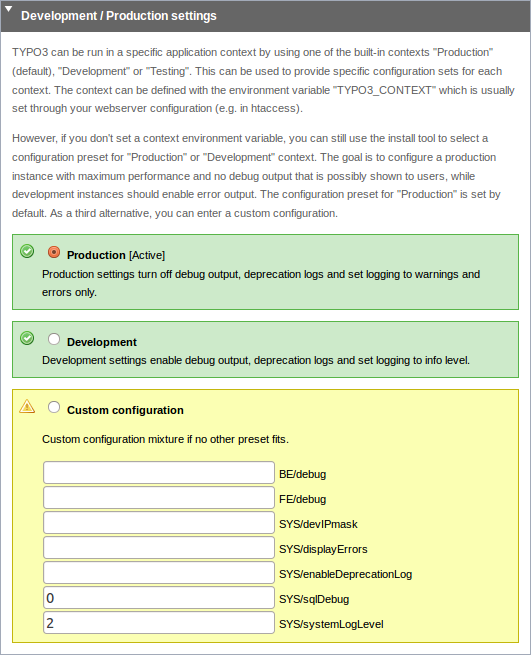
\includegraphics[width=0.8\linewidth]{Images/InstallTool/ApplicationContext.png}
			\end{figure}

		\end{column}
	\end{columns}

\end{frame}

% ------------------------------------------------------------------------------
% Improved Usability
% ------------------------------------------------------------------------------

\begin{frame}[fragile]
	\frametitle{Herramienta de Instalación}
	\framesubtitle{Usabilidad Mejorada}

	\begin{columns}[T]
		\begin{column}{.5\textwidth}

			\begin{itemize}
				\item Posición fija del menú de la izquierda al hacer scroll
					\begingroup\color{typo3red}\textbf{(1)}\endgroup
				\item Posición fija del botón "Escribir configuración" en la parte inferior
					\begingroup\color{typo3red}\textbf{(2)}\endgroup
				\item Se agrupan y ordenan las entradas de "Toda la Configuración" (se despliega una sección haciendo clic en el encabezamiento)
					\begingroup\color{typo3red}\textbf{(3)}\endgroup
			\end{itemize}

		\end{column}
		\begin{column}{.5\textwidth}

			\begin{figure}\vspace*{-0.4cm}
				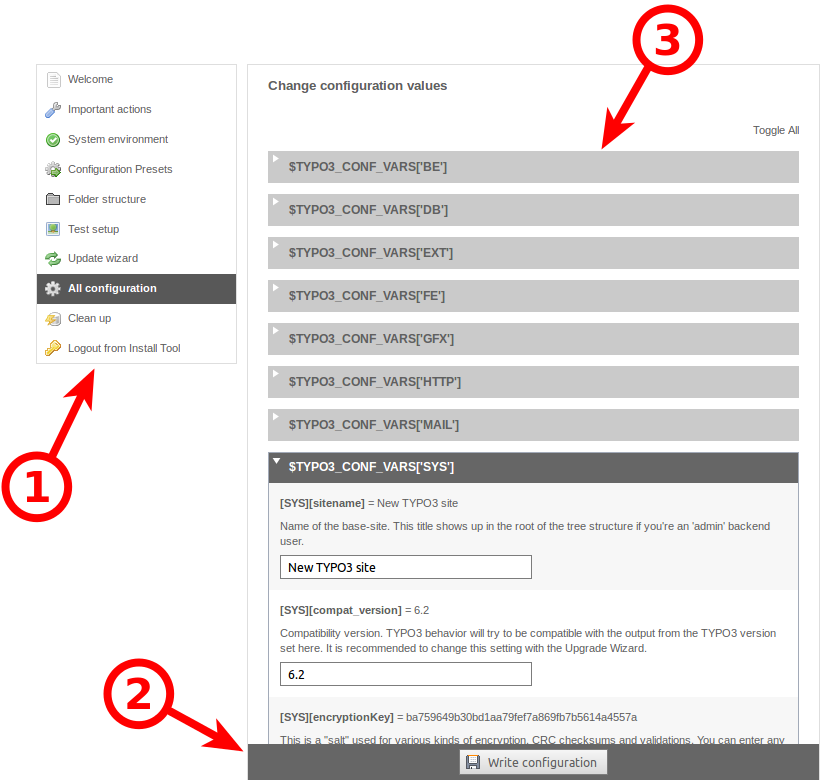
\includegraphics[width=0.8\linewidth]{Images/InstallTool/ImprovedUsability.png}
			\end{figure}

		\end{column}
	\end{columns}

\end{frame}

% ------------------------------------------------------------------------------
% Human-Friendly Error Codes
% ------------------------------------------------------------------------------

\begin{frame}[fragile]
	\frametitle{Herramienta de Instalación}
	\framesubtitle{Códigos de Error Amistosos}

	\begin{itemize}
		\item Pueden usarse palabras clave significativas para las siguientes opciones:\newline
			(TYPO3 < 6.2: sólo valores numéricos)
	\end{itemize}

	\begin{columns}[T]
		\begin{column}{.4\textwidth}
			\advance\leftskip+0.8cm

			\smaller
				\texttt{[SYS][errorHandlerErrors]}\newline
				\texttt{[SYS][exceptionalErrors]}\newline
				\texttt{[SYS][syslogErrorReporting]}\newline
				\texttt{[SYS][belogErrorReporting]}\newline
			\normalsize

		\end{column}
		\begin{column}{.6\textwidth}

			\begin{figure}\vspace*{-0.4cm}
				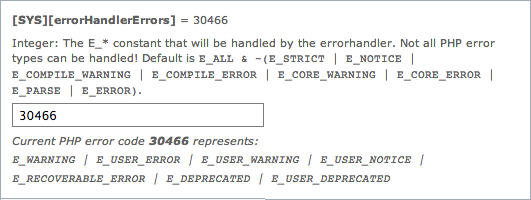
\includegraphics[width=0.9\linewidth]{Images/InstallTool/HumanFriendlyErrorCodes.png}
			\end{figure}

		\end{column}
	\end{columns}

	\vspace{0.2cm}

	\begin{itemize}
		\item Un ViewHelper Extbase \textbf{format.phpErrorCode} se encarga de la conversión a códigos de error en PHP
	\end{itemize}

\end{frame}

% ------------------------------------------------------------------------------
% Errors In Folder Structure
% ------------------------------------------------------------------------------

\begin{frame}[fragile]
	\frametitle{Herramienta de Instalación}
	\framesubtitle{Errores en Estructura de Carpeta}

	\begin{itemize}
		\item Se listan errores bajo "Estructura de Carpeta" con un símbolo (número rodeado por un círculo)
	\end{itemize}

	\begin{figure}
		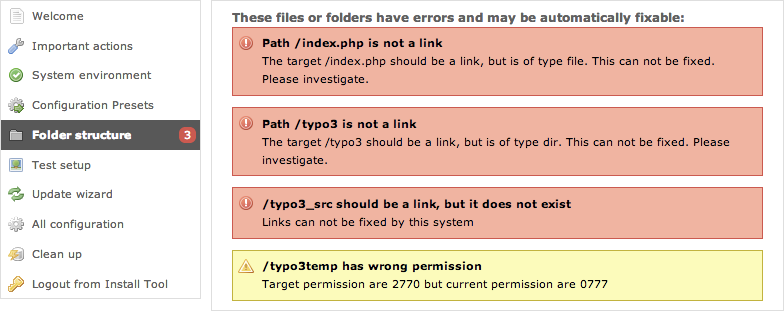
\includegraphics[width=0.95\linewidth]{Images/InstallTool/ErrorsInFolderStructure.png}
	\end{figure}

\end{frame}

% ------------------------------------------------------------------------------
% Core Updates
% ------------------------------------------------------------------------------

\begin{frame}[fragile]
	\frametitle{Herramienta de Instalación}
	\framesubtitle{Actualizaciones del Núcleo}

	\begin{itemize}
		\item El núcleo de TYPO3 se actualiza a su última versión menor con un click de botón
		\item La variable de entorno \texttt{TYPO3\_DISABLE\_CORE\_UPDATER=1} desactiva esta característica
	\end{itemize}

	\begin{figure}
		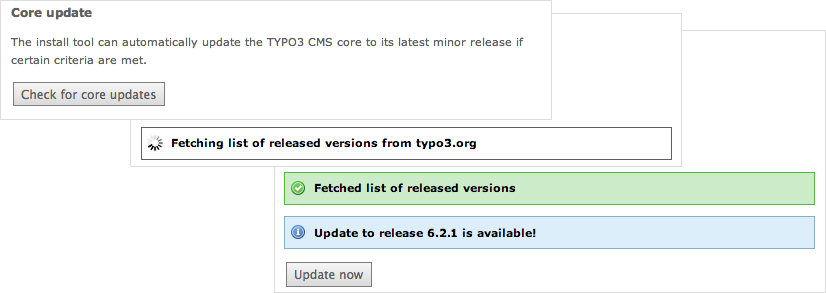
\includegraphics[width=0.95\linewidth]{Images/InstallTool/CoreUpdate.png}
	\end{figure}

\end{frame}

% ------------------------------------------------------------------------------
% Miscellaneous
% ------------------------------------------------------------------------------

\begin{frame}[fragile]
	\frametitle{Herramienta de Instalación}
	\framesubtitle{Varios (1)}

	\begin{itemize}
		\item Todos los formularios están protegidos con CSRF\newline
			  (\textit{cross-site request forgery})
		\item La Herramienta de Instalación usa una\newline
		 	  Vista Fluid Standalone simplificada
		\item Sólo se cargan las funciones TYPO3 esenciales\newline
			(\texttt{ext\_localconf.php} o \texttt{ext\_tables.php} corruptos de extensiones no pueden romper la Herramienta de Instalación nunca más)
		\item Nuevo punto de inicio:\newline
			\texttt{typo3/sysext/install/Start/Install.php}\newline
			Antes:					\tabto{3.2cm} \texttt{typo3/install/index.php}\newline
									\tabto{3.2cm} (existe una redirección desde la vieja URL a la nueva)
	\end{itemize}

\end{frame}

\begin{frame}[fragile]
	\frametitle{Herramienta de Instalación}
	\framesubtitle{Varios (2)}

	\begin{itemize}
		\item La caché desactivada asegura que la Herramienta de Instalación permanece usable, incluso si la caché contiene código PHP inválido
		\item Chequea si la opción de PHP \texttt{xdebug.max\_nesting\_level} muestra un valor de 250 o superior (el valor por defecto "100" probablemente causa problemas)
		\item "Chequeo de permisos relajado":

			\small
				Si la carpeta del directorio raíz no tiene los permisos correctos  (p.ej. "2770"),
				y no puede solucionarse esto, p.ej. porque el directorio no pertenece
				al usuario del sistema que corre la Herramienta de Instalación, el primer paso de la instalación
				se rompe.
				La opción "targetPermissionRelaxed" reduce la severidad si los permisos no son
				ideales y permite continuar con la instalación mientras puedan crearse las subcarpetas necesarias.
			\normalsize
	\end{itemize}

\end{frame}

% ------------------------------------------------------------------------------
% Miscellaneous
% ------------------------------------------------------------------------------

\begin{frame}[fragile]
	\frametitle{Herramienta de Instalación}
	\framesubtitle{Varios (3)}

	\begin{itemize}
		\item Borradas las opciones (claves) de la Herramienta de Instalación\newline
			\small(y por tanto del fichero \texttt{LocalConfiguration.php}, también):\normalsize
	\end{itemize}

	\begin{columns}[T]
		\begin{column}{.5\textwidth}
			\advance\leftskip+0.8cm
			\smaller
				\texttt{BE/loginLabels}\newline
				\texttt{BE/loginNews}\newline
				\texttt{BE/useOnContextMenuHandler}\newline
				\texttt{EXT/em\_mirrorListURL}\newline
				\texttt{EXT/em\_wsdlURL}\newline
				\texttt{EXT/extList}\newline
				\texttt{EXT/extList\_FE}\newline
				\texttt{EXT/noEdit}\newline
			\normalsize
		\end{column}
		\begin{column}{.5\textwidth}
			\smaller
				\texttt{FE/defaultTypoScript\_editorcfg}\newline
				\texttt{FE/simulateStaticDocuments}\newline
				\texttt{GFX/noIconProc}\newline
				\texttt{GFX/TTFLocaleConv}\newline
				\texttt{SYS/additionalAllowedClassPrefixes}\newline
				\texttt{SYS/caching/cacheBackends}\newline
				\texttt{SYS/caching/cacheFrontends}\newline
				\texttt{SYS/extCache}\newline
				\texttt{SYS/T3instID}\newline
			\normalsize
		\end{column}

	\end{columns}

\end{frame}

% ------------------------------------------------------------------------------

